\begin{figure}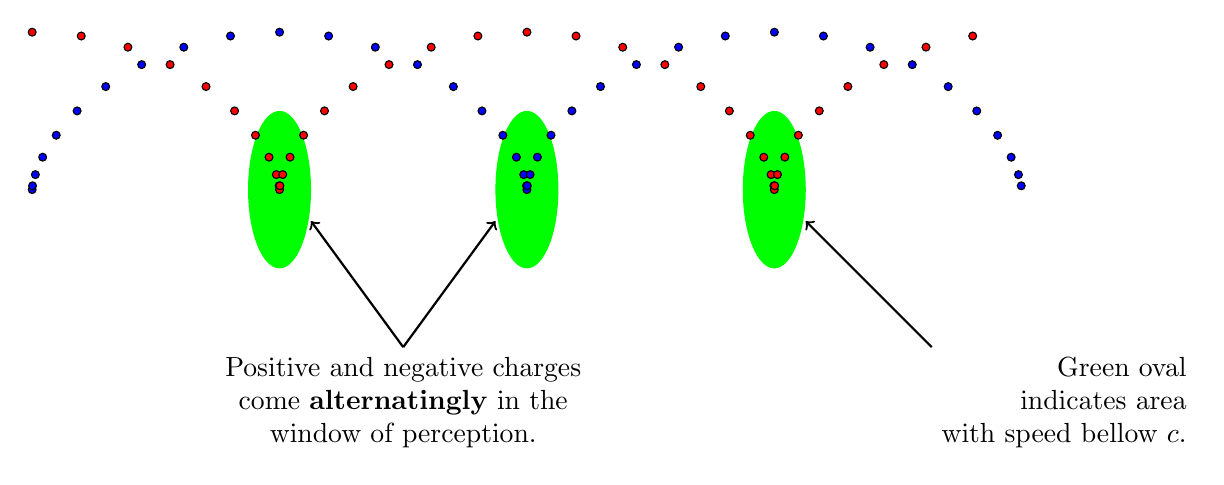
\begin{tikzpicture}[scale=1, rotate=0]

% two ornac of a photon  going through two cycloid cycle in red and blue
% with green oval to indicate the under c area

% greeen ovals
 \foreach \p in {1,...,3}
    \draw [draw = none, fill = green]
     (pi*\p,0) circle [ x radius = 0.4, y radius = 1 ];

\path
(3*pi,0) node (greenoval) {};
\draw[<-, thick] (greenoval)+(0.4,-0.4) -- ++(2,-2) node (slowspeed){}; 
\path
(slowspeed) node [below right , align=right]
{Green oval \\ indicates area \\ with  speed bellow $c$.};

\path
(1*pi,0) node (greenoval1) {}
(2*pi,0) node (greenoval2) {};
\draw[<-, thick] (greenoval1)+(0.4,-0.4) -- (1.5*pi,-2) node (alternatingly){}; 
\draw[<-, thick] (greenoval2)+(-0.4,-0.4) -- (1.5*pi,-2) node {}; 
\path
(alternatingly) node [below , align=center]
{Positive and negative charges \\ 
come  \textbf{alternatingly} in the \\ 
window of perception.};


%% red ornac
 \foreach \x in {0, 0.05,...,2}
  {
    \draw[black, fill=red] 
   ({((2*pi*\x + sin(2*pi*\x r)) },{1 + cos(2*pi*\x r) }) circle [radius=0.05];
  }


%% blue ornac
 \foreach \x in {0, 0.05,...,2}
  {
    \draw[black, fill=blue] 
   ({((2*pi*\x + sin((2*pi*\x -pi) r)) },{1 + cos((2*pi*\x -pi) r) }) circle [radius=0.05];
  }

\end{tikzpicture}\caption{Two ornac of a photon  going through two cycloid cycle in red and blue
 with green oval to indicate the under c area
\label{fig:two_ornac_cycloid_green_area}}
\end{figure}
